\documentclass{standalone}
\usepackage{tikz}

\begin{document}
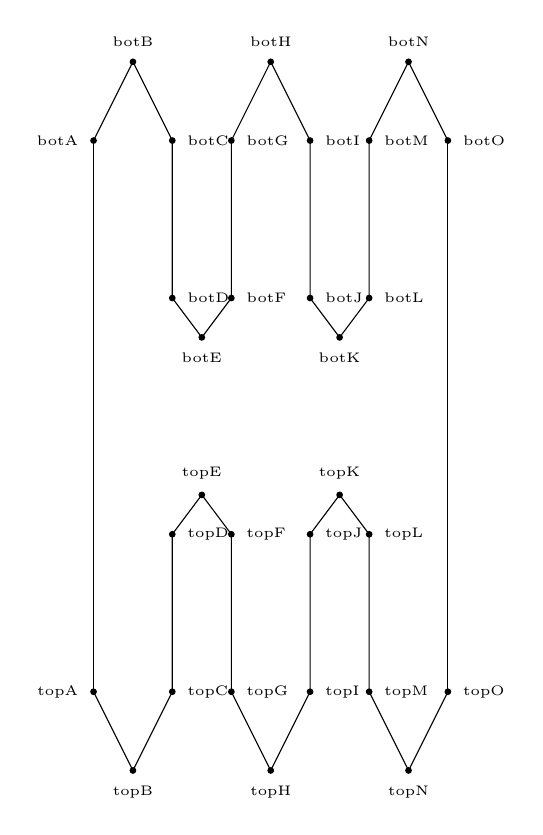
\begin{tikzpicture}
    \coordinate (topA) at (2.75, 1.5);
    \coordinate (topB) at (3.25, 0.5);
    \coordinate (topC) at (3.75, 1.5);
    \coordinate (topD) at (3.75, 3.5);
    \coordinate (topE) at (4.125, 4);
    \coordinate (topF) at (4.5, 3.5);
    \coordinate (topG) at (4.5, 1.5);
    \coordinate (topH) at (5, 0.5);
    \coordinate (topI) at (5.5, 1.5);
    \coordinate (topJ) at (5.5, 3.5);
    \coordinate (topK) at (5.875, 4);
    \coordinate (topL) at (6.25, 3.5);
    \coordinate (topM) at (6.25, 1.5);
    \coordinate (topN) at (6.75, 0.5);
    \coordinate (topO) at (7.25, 1.5);
    

    \coordinate (botA) at (2.75, 8.5);
    \coordinate (botB) at (3.25, 9.5);
    \coordinate (botC) at (3.75, 8.5);
    \coordinate (botD) at (3.75, 6.5);
    \coordinate (botE) at (4.125, 6);
    \coordinate (botF) at (4.5, 6.5);
    \coordinate (botG) at (4.5, 8.5);
    \coordinate (botH) at (5, 9.5);
    \coordinate (botI) at (5.5, 8.5);
    \coordinate (botJ) at (5.5, 6.5);
    \coordinate (botK) at (5.875, 6);
    \coordinate (botL) at (6.25, 6.5);
    \coordinate (botM) at (6.25, 8.5);
    \coordinate (botN) at (6.75, 9.5);
    \coordinate (botO) at (7.25, 8.5);
    

    % Draw 
    \draw[smooth cycle] (topA) -- (topB) -- (topC) -- (topD) -- (topE) -- (topF) -- (topG) -- (topH) -- (topI) -- (topJ) -- (topK) -- (topL) -- (topM) -- (topN) -- (topO);

    \draw[smooth cycle] (botA) -- (botB) -- (botC) -- (botD) -- (botE) -- (botF) -- (botG) -- (botH) -- (botI) -- (botJ) -- (botK) -- (botL) -- (botM) -- (botN) -- (botO);

    \draw (topA) -- (botA);
    \draw (topO) -- (botO);


    % Labeling
    \foreach \point/\position in {topA/left, topB/below, topC/right, topD/right, topE/above, topF/right, topG/right, topH/below, topI/right, topJ/right, topK/above, topL/right, topM/right, topN/below, topO/right}
        \draw[fill=black] (\point) circle (1pt) node[\position=2pt, font=\tiny] {\point};

    \foreach \point/\position in {botA/left, botB/above, botC/right, botD/right, botE/below, botF/right, botG/right, botH/above, botI/right, botJ/right, botK/below, botL/right, botM/right, botN/above, botO/right}
        \draw[fill=black] (\point) circle (1pt) node[\position=2pt, font=\tiny] {\point};
\end{tikzpicture}
\end{document}